%1. La memoria incluirá una portada portada normalizada con la siguiente información: título en castellano, título en inglés, autores, profesor director, codirector si es el caso, curso académico e identificación de la asignatura (Trabajo de fin de grado del Grado en - nombre del grado correspondiente-, Facultad de Informática, Universidad Complutense de Madrid). Los datos referentes al título y director (y codirector en su caso) deben corresponder a los publicados en web de TFG, según lo indicado en el punto 6 de la sección III de esta normativa. 
% 2. en cada apartado
% 3. La memoria constará de un mínimo de 25 páginas para los proyectos realizados por unúnico estudiant

\documentclass[12pt, a4paper, hidelinks]{article}
\usepackage[spanish, english]{babel} 	% language

% table of contents
\usepackage{tocloft}

% for sections
\renewcommand{\cftsecleader}{\cftdotfill{\cftdotsep}} 

% images
\usepackage{graphicx}
\graphicspath{ {./images/} }

% wrap around images
\usepackage{wrapfig}

% tables
\usepackage{longtable}
\usepackage{booktabs} 	% line separators

% links
\usepackage{hyperref}
\hypersetup{
	colorlinks=false
}

% bibliography
\usepackage[
backend=biber,
style=numeric,
]{biblatex}
\addbibresource{biblio.bib}



\title{\textbf{A sampler plugin for digital audio workstations}}

%\title{\textbf{Sampler plugin for digital audio workstations\\---\\ Instrumento virtual basado en samples para estaciones de trabajo de audio digital}}

%\author{Juan Chozas Sumbera}
\date{\vspace{-10ex}}

\begin{document}
	\maketitle
	\begin{center}
		\textbf{Trabajo de Fin de Grado en Ingeniería Informática}\\
		
		~\newline
		\textbf{\large{Juan Chozas Sumbera}}
		
		~\newline
		Dirigido por
		
		\textbf{Jaime Sánchez Hernández\\
		Miguel Gómez-Zamalloa Gil}
		
		
		~\newline
		
\includegraphics[width=0.5\textwidth]{logo_UCM.png}\\
		~\newline
		
		\textbf{\large{UNIVERSIDAD COMPLUTENSE DE MADRID}}\\
		
		\textbf{FACULTAD DE INFORMÁTICA}
	\end{center}

	
	
	% 2. La memoria debe incluir la descripción detallada de la propuesta hardware/software realizada y ha de contener: 
	% a. un índice, 
	% \tableofcontents % despues del resumen y antes de la intro
	\newpage

	
	% b. un resumen y una lista de no más de 10 palabras clave para su búsqueda bibliográfica, ambos en castellano e inglés, 
	\newpage
	\huge
	\textbf{Abstract}\\

	\normalsize
	Music production is at anyone's reach. Nowadays, computers, smartphones and tablets are able to run software that provides the necessary tools to compose music. Digital Audio Workstations (DAWs) are found at the more sophisticated end of the spectrum. These feature-packed programs are the type that you would find in locations ranging from the aspiring musician's personal computer to the most professional recording studio in your city. One of the most powerful characteristics of these environments is being extensible via plugins. \par	
	The sampling techniques that emerged during the end of the 20th century gifted the world with new methods of music composition. The technique that this project develops upon consists in the creation of an instrument using audio recordings as its only source of sound. The nature of the process is far from complex and it can be streamlined to provide a fast way to design a bespoke instrument. By implementing this tool as a plugin, the instrument takes the form of a loadable module that is readily accessible to anybody working on a DAW.
	
	\vspace*{\fill}
	\large
	\textbf{Key words}\\
	
	\vspace{-1em}
	\normalsize	
	\noindent music, sound, sampler, sampling, instrument, MIDI, DAW, plugin, VST, synthesizer\\

	\newpage
	\huge
	\textbf{Resumen}\\
	
	\normalsize
	Cualquier persona tiene a su alcance la producción musical. El mundo en el que vivimos esta plagado de dispositivos capaces de ejecutar programas que ofrecen todas las herramientas necesarias para componer música.	Las estaciones de audio digital son los programas que ofrecen la mayor gama de herramientas para la creación de música. Es el tipo de software que no puede faltar en los ordenadores de los músicos principiantes ni de los estudios de grabación más sofisticados. Estos entornos pueden ser enriquecidos mediante módulos externos (plugins), extendiendo la gama de utilidades que pone a disposición del usuario.\par
	A finales del siglo 20 emergieron nuevas técnicas de muestreo, nuevas maneras de producir música utilizando grabaciones de sonido. Este proyecto utiliza estas técnicas de base para ofrecer una manera rápida de crear un instrumento a medida que utiliza regiones de una muestra para producir sonido. El proceso es sencillo por naturaleza y se puede implementar de forma eficiente para hacer un proceso sin demoras innecesarias del diseño de un instrumento basado en muestras. La implementación en forma de plugin hace que el instrumento sea accesible para todo el que trabaje con una estación de audio digital.

	
	\vspace*{\fill}
	\large
	\textbf{Palabras clave}\\
	
	\vspace{-1em}
	\normalsize	
	\noindent música, sonido, muestra, muestreo, instrumento, MIDI, DAW, plugin, VST, sintetizador
	
	
	
	\newpage
	% a. un índice, 
	\tableofcontents


	% c. (25 pg entre c y d) una introducción con los antecedentes, objetivos y plan de trabajo, 
	\newpage
	\section{Introduction}
	\subsection{Background}
	\subsubsection{Sampler history}
	The technique of sampling dates back to the 1960s when recordings were captured on tape. Thanks to a hardware design that made contact between the playback head and different sections of a moving tape, musicians could play the distinct recordings on keyboards of instruments such as the Mellotron. During the 1980s, the popularity of drum machines increased significantly. Many drum machines were sample-based, i.e. they created sounds using digitally stored samples, whereas the alternative was to synthesize sound in an analog fashion. In 1988, the first Music Production Center (MPC) by Akai was made available to the public: a sample-based music workstation that was capable of arranging samples of all lengths in its sequencer to produce full fledged music tracks without the need for additional instruments or hardware. In a recipe for music, an MPC could be the only ingredient, reaching a vast number of musicians because of its affordability in comparison to previous means of music production. It is a tool that gave artists a new way to create music, a technique that has been a foundation to several genres and highly influential to music as a whole.\par
	

	\subsubsection{Pulse-Code Modulation}
		\begin{figure}[h]
		\centering
		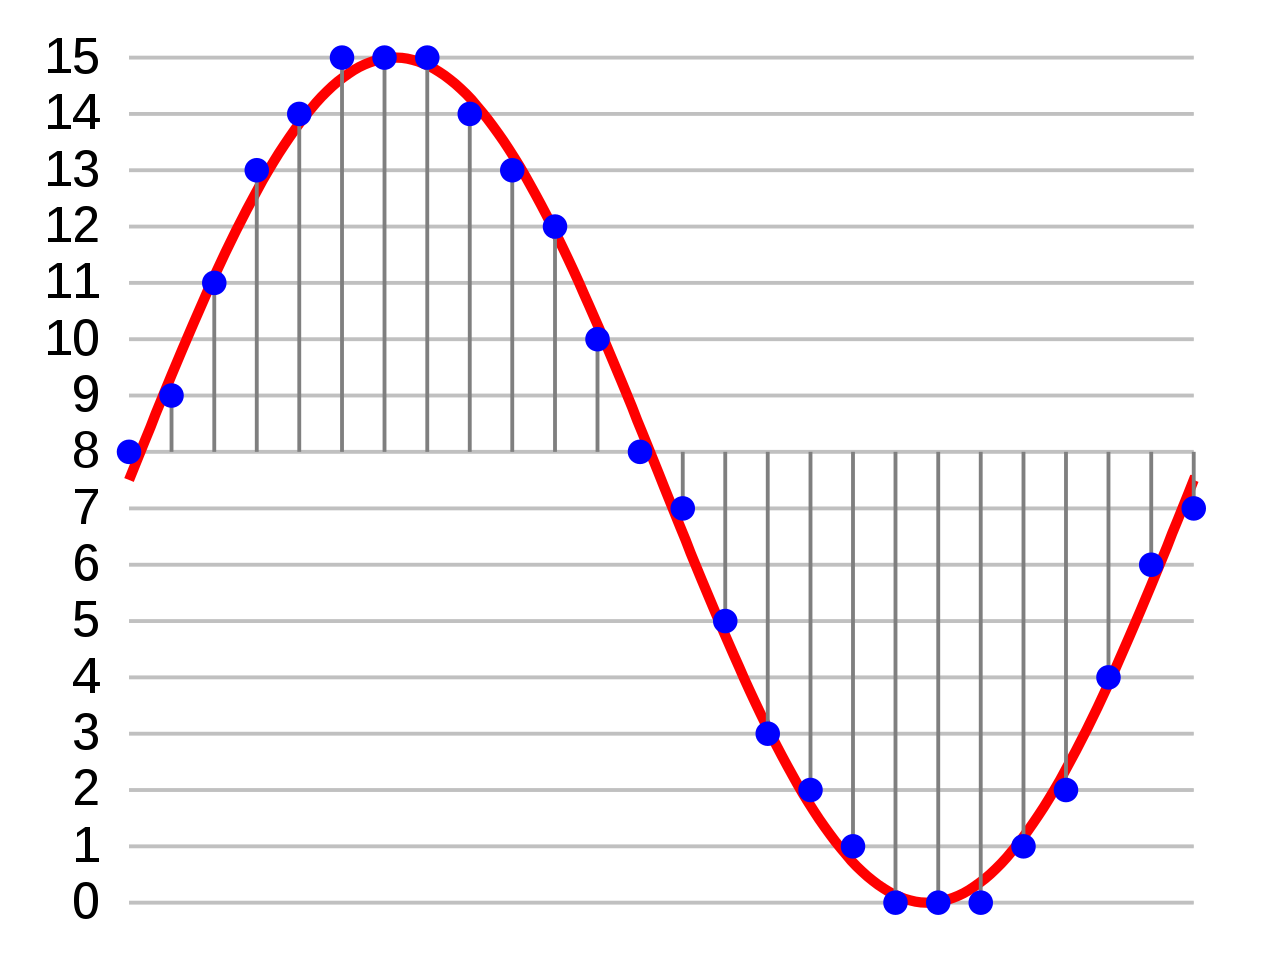
\includegraphics[width=0.5\textwidth]{pcm.png}
		\caption{Linear pulse-code modulation at 4 bit depth. \cite{pcm_img}}
		\label{fig:pcm}
	\end{figure}
	The method that makes sampling a possibility is Pulse-Code Modulation (PCM for short). Dating back to the 1930s, it consists of the digital representation of analog signals, and is subject to two parameters: sampling rate and bit depth. This technique processes an input analog signal by making readings at equidistant intervals. Commonly referred to as samples, these readings are what the resulting digital representation will be composed of. The sampling rate refers to how often samples will be read from the analog signal, and the bit depth indicates the amount of bits with which to describe each sample. Every time an analog reading is being converted into a digital sample, it is rounded to the nearest integer value in the range determined by the bit depth. This rounding process, visible in Figure \ref{fig:pcm} is known as quantization. Since samples are encoded to integers in binary, the levels to which they can be quantized are uniformly distributed. This describes the method of Linear PCM (LPCM), a sub-method of PCM that is used for audio CDs and the popular formats WAVE and AIFF, among other applications.\par
	

	
	\subsubsection{Modern music production} 	
 	In a world of highly complex information systems, digital music production has been developed thoroughly. When it comes to modern music composition, Musical Instrument Digital Interface (MIDI from now on) protocols provide grounds for an alternative to regular, "analog" instruments. This standard erects a bridge for communication between digital instruments and computers, providing the world of digital music production with the tangible interfaces of normal instruments. The MIDI standard provides, among many other features, a communications protocol that encodes music events. This manifests in the form of messages which describe data such as the pressing, releasing, and velocity of musical notes. 	
	 	
 	A digital audio workstation (DAW from here on out) is a software environment for music production. These workstations revolve around MIDI, which provides an encoded language for musical notes. See Table \ref{table:notes} for a table of the syllabic and alphabetical equivalents of musical notes. Note-related MIDI messages always store data regarding the note subject to the event. 
 	\par
	\begin{table}[h]
		\centering
		\begin{tabular}{c c}
			Syllabic & Alphabetical \tabularnewline
			\midrule
			Do  & C \tabularnewline
			Re  & D \tabularnewline
			Mi  & E \tabularnewline
			Fa  & F \tabularnewline
			Sol & G \tabularnewline
			La  & A \tabularnewline
			Si  & B \tabularnewline
		\end{tabular}
		\caption{Musical notes in syllabic and alphabetical form}
		\label{table:notes}
	\end{table} 
	One can have an extensive range of digital synthesizers, samplers, and effect chains all working simultaneously in a DAW, the type of software that provides a playground that routes audio between racks of components and effects, making music production a possibility to anyone that owns a computer. DAWs have an element called a sequencer, which serves as a sort of digital equivalent to sheet music. The sequencer is where producers draw out musical events, placing small rectangles on a grid to represent the notes, their length, and their duration. The arrangements of events are then encapsulated in what are called patterns. These patterns can be applied to instruments, such as synthesizers, or samplers, to trigger the sounds they produce. Patterns can be drawn out manually, auto generated, or recorded in real time with a MIDI controller. Auto generated patterns consist of filling a set length of time with notes separated by constant intervals, so as to mimic the timing of a metronome, for example. Patterns that are recorded in real time are made with the DAWs recording function, which is activated to record MIDI events from a controller. \par 

	When recording patterns, incoming MIDI events are timestamped to then be displayed in chronological order and resemble the translation of the user's input. A user may have an instrument loaded during this recording period, so the user can know what sounds are being produced. It is important to highlight what is captured by the DAW is a sequence of MIDI events, not the actual sounds being produced by the instrument, meaning that a pattern is just a sequence of data, void of sound until an instrument that can process the events is associated to it. More so, since patterns are composed of MIDI events meant to trigger responses from instruments, there is no binding between them and instruments, and a pattern made for one instrument can perfectly be used for another. \par 
	
	The relevant events associated to the pattern building process are: note-on events, the signal that a note has been pressed; note-off events, the signal that a note has been released. The subtraction of the timestamps associated to these two events determines how long a note is held down. A musical note is associated to note-on and note-off events, having the note and octave being encoded as an integer in the range of $[0, 127)$. In addition, associated to note-on events is an element called velocity, which is a measure of the intensity of the note. The velocity of a note is sometimes processed by instruments to generate softer or stronger sounds. Some samplers use note velocity to trigger a sample from a set, i.e. a lower intensity recording of a snare drum for lower velocities as opposed to a sample of a powerful snare drum hit when the velocity is a higher range.
 	\par
 	
	DAWs can be extended with plugins in the form of effects or instruments. The former normally have a sound-based input-output relation with the DAW, meanwhile instruments will take MIDI messages and produce a sound as an output. The most common standard for plugins is Virtual Studio Technology (VST), created by a german company called Steinberg. VST plugins have multi platform support on major operating systems, however, plugins must be exported for a target operating system, i.e. a VST plugin that is exported for Windows will not work on Mac OS or Linux. A possible VST plugin could be a sine wave based instrument, for example. The wave's frequency will depend on the key being pressed, and the force applied to the key will dictate the amplitude of the wave. This plugin, although simple, could be considered a synthesizer. A sampler is a synthesizer that uses samples rather than oscillators to produce sound.  The sources of the sounds it produces are samples, which can be described as clips of audio that are stored in a digital format within the sampler's memory. You're likely to find that hardware and software samplers offer sets of "stock" samples that are loaded by default. The option to load samples from an external source such as an SD card is also common, just like recording external input from a recording device such as a microphone. As is the case with non sample based synthesizers, there are several ways that the samples can be manipulated.\par
	
	\subsubsection{Sampling technique}
	The key concept of sampling techniques is to modify and manipulate audio samples to create sounds. Many types of transformations can be applied to samples in order to drastically change the way they sound, although products that sound far different to the source sample are not always the objective. A sample can be manipulated by delimiting subsections within it, so as to create separated sub-samples that can be treated as individual notes. This process is colloquially referred to as \textit{chopping} the sample, resulting in a set of \textit{chops}, the sub-samples obtained from the main sample. \par
	Another way to manipulate a sample is via \textit{envelopes}, which dictate the way a sound changes over time. Envelopes affect playback every time it is triggered, and are commonly composed of four parameters. The first one  comes into play upon note-on events, i.e. on a key press: \textit{attack}, describing the time it takes for the sound's level to rise from zero to its peak. Next, \textit{sustain} is the level at which the sound will hold until a note-off event, i.e. when a key is released. \textit{Decay} depends on sustain, and it describes the time it will take for the level to go from peak to sustain. Finally, \textit{release} is the tail end of the envelope. Starting on note-off events, it describes the time it will take to reach zero level from sustain level. These four concepts form the acronym ADSR, and can be pictured as a plot of level against time in Figure \ref{fig:envelope}. You may have noticed that three of the parameters refer to a time measure, whereas sustain refers to a level. \par
	
	
	\begin{figure}[h]
		\centering
		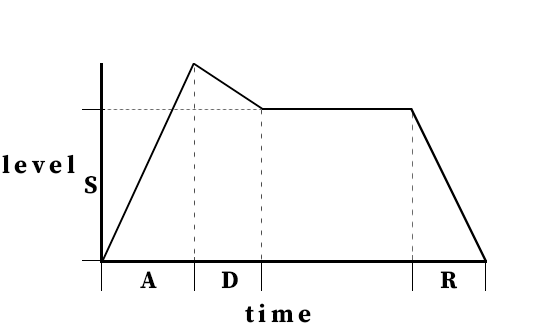
\includegraphics[scale=0.4]{envelope.png}
		\caption{ADSR parameters in envelopes}
		\label{fig:envelope}
	\end{figure}
	
 	The entity that is the sample based instrument is what holds and modifies the configuration that revolves around a main sample. It knows where to find the main sample, where each subsection starts and ends, and what the envelope parameters are set to for each chop. The sampler is equipped for playback, and is configurable in the way sounds interact as they are triggered. \par 
 	A parameter that can be found in most instruments is termed \textit{polyphony}, a measure that limits the playback at any moment to a particular number of notes. Polyphony is commonly described with an arbitrary number of \textit{voices}: an instrument with 3 voices can play at most 3 sounds at a time.\par
 	Furthermore, a series of effects may be applied to the sample in order to modify the sound that is output. Filters and compressors are some of the most common effects you may come across. Filters eliminate frequencies from the sound. Compressors apply reduction to the sound when the level crosses a certain threshold. Being applicable to any source of sound, these types of effects are most likely included with any arbitrary DAW, although they are sometimes also found within samplers.

	
	\newpage
	\subsection{Motivation}
	Modern DAWs have built in samplers or similar tools that allow a user to sample sound and directly manipulate it so as to employ sampling techniques. In most cases, these tools are more than capable of providing the means to translate these techniques into action, however, depending on the DAW, you may be hindered due to the workstation's design. Whether it be the user interface, the imposed workflow, or the minimum amount of steps required to reach your sampling goals, it is likely that the process involves inconveniences.\par
	 
	Personally, I find that there are a minimum of three steps to achieve a usable sampler configuration. First, a main sample must be loaded. Second, a number of chops are delimited in the bounds of the main sample. Third comes the assignment of chops to MIDI notes, in other words, the mapping of sample subsection playback to a controller's keys. These steps are a prerequisite to playing chops on a controller, or to lay notes out within the DAW's sequencer. At this stage, the user can experience the instrument and judge whether it is necessary to take a step back and make adjustments, for example, shifting the start time of a chop, creating/deleting a chop, or moving the trigger note to another of higher convenience. All of this implies that the design of a sampler instrument is an iterative process, and that the user may keep reforming it in several ways to fit the necessities of the creative process in musical composition. \par 
	
	Since the essential number of steps and functions required to obtain a usable instrument are few, there is room for improvement in comparison to the process that takes place when using a DAW's default tools. By focusing on the indispensable functions and actions, the process can be simplified to provide a fast way of putting together a sample based instrument. Hindrances such as overloaded user interfaces are eliminated, leaving out the buttons and functionalities that are seldom used. \par
	
	By implementing the instrument as a VST plugin, a vast number of DAWs become candidates for the inclusion of this plugin and the streamlined process of sampling. Any DAW's inherent limitations and/or hindrances would no longer be obstacles when it comes to creating a sample based instrument. This way, the instrument would be attachable to the majority of workstations and optimized for the application of sampling techniques required to translate an idea into sound.
	  

	
	
	

	\newpage
	\subsection{Objectives}
	% TODO creación de un instrumento personalizado mediante la inclusión de lo estrictamente necesario: 
	For the simple implications of sampling techniques, the means by which you achieve a minimum setup with which you can play around and manifest ideas should be straightforward. The aim is to reduce the amount of user interaction required to reach a usable sample based instrument. To do so, I will downsize in the features that any arbitrary DAW has to offer, including only those that are strictly necessary. This translates to the reduction of hindrances that may arise when there is an excess amount of functionality that is rarely used.  By implementing the instrument as a VST plugin, I aspire to build an accessible sample based instrument optimized for the application  of sampling techniques. %This means that the user will be able to load, chop, and play samples with speed and ease in a reduced sequence of actions. In addition, the user should also be able to make fast corrections and tweaks to further develop the instrument. 
	\par
	The capabilities of the sampler can be summarized to four key functionalities:
	\begin{itemize}
		\item Capacity to load an audio clip as the main sample                     % TODO MORE THAN ONE SAMPLE?
		\item Manual chopping and automatic chopping with a peak detection algorithm
		\item Visual representation and audio preview of the main sample and its chops
		\item Editable envelope parameters for each chop                            % TODO chop pan? vol? filters?
	\end{itemize}


	% TODO FUNCIONES A INCLUIRSE 
%	visualización visual y sonora del sample y sus cortes
%	lista de cortes y a donde estan mapeados
%	deteccion de picos para creacion "automática" de cortes
%	opciones de playback (adsr, polyphony)
		
	
	\newpage	
	\section{Plugin design}
	% TODO reiterar las funciones a incluirse pero mediante elementos GUI y lo necesario de la interfaz (?)
	
	
	\newpage
	\section{Implementation}
	\subsection{JUCE framework}
	%intro juce, support for plugins, extensive tutorials and examples
	To implement the sampler, I used an application framework called JUCE\cite{juceweb}. It has cross-platform support and is written in C++. The amount of documentation and tutorials available online was enough to convince me that I would need nothing else to implement the majority of the instrument.
	
	% how does juce work? what does it offer? object oriented, event driven 
	JUCE makes use of the object oriented capabilities of C++ to present a wide array of classes and utilities. It offers the building blocks to application development with a reasonably gentle learning curve that discards the need to reinvent the wheel. These utilities help with tasks that range from audio playback, to event driven data structures, to the design of user interfaces. Furthermore, the framework is in line with the event-driven paradigm, which makes the development of action based applications a simple and efficient task. As stated, the documentation is vast and there are numerous descriptive tutorials. On top of that, at the programmers disposal are more than 70 example applications that showcase the several features the framework has to offer. 
	
	% linux - windows tradeoff, makefile & freedom from ide VS vst export only on windows and vs2017/codeblocks
	The Projucer is JUCE's cross-platform application that allows for the creation, management and configuration of JUCE projects. To enable development on Linux, for example, one can add a Makefile exporter to their project. The Projucer will create an architecture specific Makefile that links external libraries and builds the application. The templates offered from which to start new projects include GUI Application, Animated Application, Console Application, Audio Application, Audio Plugin, and Static Library and Dynamic Library. Each of these archetypes are configurable in distinct ways, and are initialized to include the fundamental code inherent to the nature of the application. For Audio Plugin projects, the Projucer can export several plugin formats, such that one build process compiles and exports the plugin formats that the project is configured to build. The formats include VST and Standalone Application, among other less relevant plugin formats. Building a Standalone Application allows for the usage of the plugin without the need of a DAW. Building VST plugins is only supported on Windows, which means that for development on Linux, one can only test the build in an isolated, standalone application, void of connections to a DAW. \par
	
	% 0. explain components and structure of project
	The Projucer's base audio plugin project provides fundamental code containing two classes. The dichotomy encourages the separation of the audio processing logic from the GUI side of the plugin. The \textit{PluginProcessor}, as the name suggests, is the audio processing heart of the application. This class extends the \textit{AudioProcessor} class, a base class for audio processing. This is where tasks such as MIDI connection management and audio rendering take place. The \textit{PluginEditor} extends from the \textit{AudioProcessorEditor} class, and is intended to be the GUI. It is the place where interaction with GUI and all on screen visualizations are created and managed. Unlike the \textit{AudioProcessor} class, which inherits from no other, the \textit{AudioProcessorEditor} class extends from the \textit{Component} class. This is the base class for all user interface objects that can be visualized. The \textit{Component} class has two virtual functions that are to be overridden by any class derived from it: \texttt{paint()}, the function that dictates the on screen layout of the component; \texttt{resized()}, which contains reactionary logic for when the component is resized. Both functions are callbacks, which means they are invoked automatically upon triggering events.\par
	
	
	\newpage	
	\subsection{Audio preview}
	% TODO (REVEIW): Visualización con AudioThumbnail && AudioTransport, Sources, como se combina todo para leer & reproducir sonido
	
	The first step in developing the sampler consisted in loading an audio file. With the help of the \textit{Draw audio waveforms} tutorial \cite{audiothumbnail}, I was quickly able to identify the classes I would need to load, and, additionally, display a visual representation of an audio file. For starts, a \textit{FileChooser} object is used to create a dialog box that selects files or folders. One can limit the formats allowed for selection by specifying semicolon separated regular expressions in its constructor. Using the string \texttt{"*.wav"} as the \texttt{filePatternsAllowed} parameter will only allow users to select WAVE files, for example. The class offers several member functions named with "\texttt{browseFor}" as a prefix, and \texttt{browseForFileToOpen()} opens a dialog box to select a file for opening, returning a boolean value that indicates whether the user selected a file or not. In the former case, the FileChooser's \texttt{getResult()} function will return the \textit{File} object that was selected. \par
	The class that would provide the visual representation of the audio file is the \textit{AudioThumbnail} class. It works hand in hand with the \textit{AudioThumbnailCache} class, which serves as a cache memory of audio file representations. Together, they store and print waveform representations of audio files. I created a separate class \textit{SamplerThumbnail} to bundle the \textit{AudioThumbnail} object and its related objects and functions into a separate component. For the thumbnail view to load the audio file, I created a public function \texttt{setFile(const File\& file)} within the \textit{SamplerThumbnail} class. Within \texttt{setFile}, the audio file is loaded with the \texttt{setSource(FileInputSource* newSource)} function of \textit{AudioThumbnail}. The \textit{FileInputSource} object can be created from the \textit{File} received from the \textit{PluginEditor} by passing the file as the only parameter to the constructor of a \textit{FileInputSource} object. With this done, the \textit{AudioThumbnail} will load the waveform representation of user-selected audio files.\par
	

	% PLAYBACK
	Audio playback is achieved through the \textit{AudioTransportSource} class. It inherits from the \textit{AudioSource} class, which is a base class that enables continuous audio playback. The \textit{AudioTransportSource} is used because it implements can be positioned, played, paused, and stopped. These features are useful for previewing the initially loaded sample. Audio subsection playback is handled differently, and will be discussed later on. The connection of audio files to the \textit{AudioTransportSource} object is achieved via \textit{AudioSource} subclasses. In this case, an \textit{AudioFormatReaderSource}. The processor stores an instance of \textit{AudioFormatReaderSource} in \texttt{currentAudioFileSource}, and in \texttt{transportSource} an instance of \textit{AudioTransportSource}. \textit{AudioFormatReaderSource} objects of this class obtain streams of sound from \textit{AudioFormatReader} objects, which source their sound from audio file streams. Every time a user opens a file successfully, a function \texttt{loadFileIntoTransport(const File\& file)} is executed. This function will stop the \textit{AudioTransportSource} from continuing playback, and proceed to change the source. To do this, a new \textit{AudioFormatReader} object is created for \texttt{file}. This is done through an \texttt{AudioFormatManager} object, which is used to keep a list of the formats that are to be accepted by the application. It includes a method called \texttt{AudioFormatReader* createReaderFor (const File\& file)}, which returns a pointer to the \textit{AudioFormatReader} that is necessary for the creation of an \textit{AudioFormatReaderSource}. If \texttt{createReaderFor} fails, it returns a null pointer, so the following steps are only taken in cases where the pointer is not null. The \texttt{currentAudioFileSource} pointer is reset to the new reader source, and the \texttt{transportSource}'s new source is set with \texttt{setSource}.\\
	All of these instances and connections lead to a functional way to play audio, however, there still is the need to connect the \texttt{transportSource}'s interface to GUI elements. The \textit{AudioTransportSource} class extends \textit{ChangeBroadcaster}, which allows for event driven reactivity to the state of the \textit{transportSource} object. To aid in the process, an \texttt{enum TransportState} is declared to include the states of \texttt{Stopping}, \texttt{Stopped}, \texttt{Starting}, \texttt{Playing}, \texttt{Pausing}, and \texttt{Paused}. Buttons layed out in the application will change a private variable \texttt{TransportState state} to \texttt{Starting}, \texttt{Stopping}, and \texttt{Pausing} to invoke \texttt{transportSource.start()} or \texttt{transportSource.stop()}. By executing these methods of the \texttt{transportSource}, every object that extends \textit{ChangeListener} that has been added to the \texttt{transportSource}'s list of listeners will be notified of a change. This notification manifests by invoking the callback function \texttt{void changeListenerCallback (ChangeBroadcaster* source)}, which is a virtual function that must be implemented by any class that extends \textit{ChangeListener}. The plugin editor extends this class and adds itself to the \texttt{transportSource}'s listener list with the following instruction: \texttt{transportSource.addChangeListener(this);}. In the \texttt{changeListenerCallback} function, the source of the event is checked by comparing references like so:
	\begin{verbatim}
	void changeListenerCallback (ChangeBroadcaster* source) override
	{
	if (source == &transportSource)
	{...
	\end{verbatim}
	Inside the conditional block, the transport state is updated once more, and the GUI is synchronized in accordance to the next transport state, for example, when \texttt{Starting}, the state transitions to \texttt{Playing}, changing the play button's text to "Pause" and enabling the stop button. \par
	
	
	
	\newpage
	\subsection{Subsection management}
	% TODO Chop list & settings: ADSR, MIDI learn, poliphony

	\textit{TODO:}
	\textit{Explain connection to chop list. link to table tutorial.}\par
	
	\textit{	midi learn and chop parameters. polyphony}
	
	
	\newpage
	\subsection{Peak detection}
	% TODO Aubio para la detección de picos y conexión mediante Projucer
	% projucer include external libraries, peak detection w aubio
	\textit{	aubio external library for peak detection. projucer configuration and calling the C code from C++}
	\par
	
	
	
	
	\newpage
	\subsection{Audio playback}
	% TODO Synthesizer: implementación de SamplerVoice & SamplerSound, procesamiento de mensajes MIDI
	% step 5: playback with midi controller: sourcereaders, synths, midi in processblock, samplerate of sample, vst debugger
	\textit{	synthesizer explained in voices, sounds. midi message detection in processblock }
	\par
	
	
	
	
	% d. (25 pg entre c y d) resultados y discusión crítica y razonada de los mismos, con sus conclusiones,
	\newpage
	\section{Results}
	
	
	


	\newpage
	\subsection{Conclusion}
	Having no experience in digital audio processing, I have to say that the JUCE framework made the process straightforward and easy to grasp.

\textit{TODO}
\textit{	juce's tutorials and example code allow for fast understanding of the framework}

\textit{	very powerful and capable of building audio applications}

\textit{translate}
	
		
	\newpage
	% e. bibliografía.
	\section{Bibliography}
	\printbibliography
	
\end{document}